\chapter{Systems Integrator Tender and Scoring Matrix}

\section{Overview}

This chapter outlines the procurement strategy for selecting a systems integrator capable of delivering our world-class immersive facility. The tender process ensures competitive proposals while maintaining the highest standards of technical excellence.

\section{Tender Scope}

\subsection{Project Deliverables}

\begin{requirement}{TEND-001}{Full turnkey solution from design through commissioning}

The selected systems integrator shall provide:

\begin{enumerate}
    \item \textbf{Detailed Design}: Complete technical drawings and specifications
    \item \textbf{Equipment Supply}: All hardware and software components
    \item \textbf{Installation}: Professional installation of all systems
    \item \textbf{Integration}: Seamless integration of all subsystems
    \item \textbf{Testing}: Comprehensive testing and validation
    \item \textbf{Training}: Operator and maintenance training
    \item \textbf{Documentation}: Complete as-built documentation
    \item \textbf{Warranty}: Minimum 2-year comprehensive warranty
    \item \textbf{Support}: Ongoing maintenance options
\end{enumerate}

\subsection{Technical Requirements Summary}

\begin{table}[H]
\centering
\begin{tabularx}{\textwidth}{@{}lX@{}}
\toprule
\textbf{System} & \textbf{Key Requirements} \\
\midrule
Display & 6-sided, 8K resolution, 6-user stereoscopic \\
Compute & 32+ GPUs, real-time ray tracing capable \\
Audio & 128-512 channel Wave Field Synthesis \\
Tracking & Sub-millimetre optical, 240Hz update \\
Volumetric & 64 cameras, real-time reconstruction \\
Infrastructure & Full redundancy, 99.9\% uptime \\
\bottomrule
\end{tabularx}
\caption{High-level technical requirements}
\end{table}

\section{Tender Process}

\subsection{Timeline}

\begin{figure}[H]
\centering
\begin{tikzpicture}[x=0.8cm, y=0.8cm]
    % Timeline
    \draw[thick, ->] (0,0) -- (16,0);

    % Milestones
    \foreach \x/\event/\duration in {
        0/{RFP Issue}/0,
        2/{Questions Due}/2,
        3/{Answers Issued}/1,
        5/{Proposals Due}/2,
        7/{Clarifications}/2,
        9/{Shortlist}/2,
        11/{Presentations}/2,
        13/{Selection}/2,
        14/{Contract}/1,
        15/{Kickoff}/1
    } {
        \draw[thick] (\x,0) -- (\x,0.3);
        \node[above, rotate=45, anchor=west] at (\x,0.3) {\small\event};
        \node[below] at (\x,-0.3) {\tiny Week \x};
    }

    % Phases
    \draw[dreamlabPrimary, ultra thick] (0,-1) -- (5,-1) node[midway, below] {Tender Period};
    \draw[dreamlabAccent, ultra thick] (5,-1) -- (13,-1) node[midway, below] {Evaluation};
    \draw[dreamlabSecondary, ultra thick] (13,-1) -- (15,-1) node[midway, below] {Award};

    \node[below] at (8,-2) {\textbf{15-Week Tender Timeline}};
\end{tikzpicture}
\caption{Procurement timeline from RFP to contract award}
\end{figure}

\subsection{Tender Requirements}

\begin{requirement}{TEND-002}{Comprehensive proposal addressing all technical and commercial aspects}

Proposals must include:

\begin{enumerate}
    \item \textbf{Executive Summary}: Overview of approach and key differentiators
    \item \textbf{Technical Proposal}: Detailed response to each requirement
    \item \textbf{Project Plan}: Timeline with key milestones and dependencies
    \item \textbf{Team Structure}: Key personnel and their qualifications
    \item \textbf{References}: Similar projects completed successfully
    \item \textbf{Commercial Proposal}: Detailed pricing breakdown
    \item \textbf{Risk Assessment}: Identified risks and mitigation strategies
    \item \textbf{Value Engineering}: Optional enhancements or alternatives
\end{enumerate}

\section{Evaluation Criteria}

\subsection{Scoring Matrix}

\begin{table}[H]
\centering
\begin{tabularx}{\textwidth}{@{}lXr@{}}
\toprule
\textbf{Criterion} & \textbf{Description} & \textbf{Weight} \\
\midrule
Technical Capability & Meeting/exceeding specifications & 35\% \\
Experience & Track record in similar projects & 20\% \\
Project Management & Approach, timeline, risk management & 15\% \\
Innovation & Creative solutions and future-proofing & 10\% \\
Support \& Maintenance & Warranty terms and ongoing support & 10\% \\
Commercial & Total cost of ownership & 10\% \\
\midrule
\textbf{Total} & & \textbf{100\%} \\
\bottomrule
\end{tabularx}
\caption{Tender evaluation scoring matrix}
\end{table}

\subsection{Technical Capability Assessment (35\%)}

\begin{figure}[H]
\centering
\begin{tikzpicture}[scale=0.8]
    % Spider chart
    \def\categories{Display,Compute,Audio,Tracking,Integration}
    \def\scores{4,5,3,4,5} % Example scores out of 5

    % Draw grid
    \foreach \i in {1,...,5} {
        \draw[gray!30] (0,0) -- (90+72*\i:3);
    }
    \foreach \r in {1,2,3} {
        \draw[gray!30] (90:{\r})
            \foreach \i in {1,...,5} {
                -- (90+72*\i:{\r})
            } -- cycle;
    }

    % Draw axes
    \foreach \i/\cat in {0/Display,1/Compute,2/Audio,3/Tracking,4/Integration} {
        \draw[thick] (0,0) -- (90+72*\i:3);
        \node at (90+72*\i:3.5) {\cat};
    }

    % Plot scores
    \draw[dreamlabPrimary, ultra thick, fill=dreamlabPrimary!20]
        (90:2.4) -- (162:3) -- (234:1.8) -- (306:2.4) -- (378:3) -- cycle;

    \node[below] at (0,-4) {\textbf{Technical Capability Scoring}};
\end{tikzpicture}
\caption{Multi-dimensional technical assessment}
\end{figure}

Detailed scoring for technical capability:

\begin{itemize}
    \item \textbf{Display System (20\%)}: Resolution, multi-user capability, technology choice
    \item \textbf{Compute Platform (20\%)}: GPU specifications, clustering approach, software
    \item \textbf{Audio System (20\%)}: WFS implementation, channel count, integration
    \item \textbf{Tracking/Capture (20\%)}: Accuracy, latency, volumetric capability
    \item \textbf{System Integration (20\%)}: Synchronisation, unified control, reliability
\end{itemize}

\section{Qualification Requirements}

\subsection{Mandatory Criteria}

\begin{requirement}{TEND-003}{Bidders must meet all mandatory qualification criteria}

\begin{enumerate}
    \item \textbf{Financial Stability}:
        \begin{itemize}
            \item Minimum £10M annual turnover
            \item Positive trading history (3 years)
            \item Professional indemnity insurance £5M
        \end{itemize}

    \item \textbf{Technical Expertise}:
        \begin{itemize}
            \item ISO 9001:2015 certification
            \item Manufacturer authorisations
            \item Certified project managers
        \end{itemize}

    \item \textbf{Experience}:
        \begin{itemize}
            \item 3+ similar installations completed
            \item Projects >£2M value
            \item Multi-user immersive systems
        \end{itemize}

    \item \textbf{Resources}:
        \begin{itemize}
            \item UK-based support team
            \item 24/7 emergency response capability
            \item Dedicated project team
        \end{itemize}
\end{enumerate}

\subsection{Preferred Qualifications}

\begin{itemize}
    \item Previous CAVE/immersive room experience
    \item Partnerships with key manufacturers
    \item Research facility experience
    \item Innovation awards or recognition
    \item Environmental certifications
\end{itemize}

\section{Potential Suppliers}

\subsection{Systems Integrators}

\begin{table}[H]
\centering
\begin{tabularx}{\textwidth}{@{}lXl@{}}
\toprule
\textbf{Company} & \textbf{Strengths} & \textbf{Location} \\
\midrule
ST Engineering Antycip & UK CAVE expertise, Leeds HIKER & UK \\
Mechdyne Corporation & Multi-viewer pioneer, global leader & USA/UK \\
Virtalis & UK-based, research focus & UK \\
Holovis & Immersive attractions, innovation & UK \\
Digital Projection & Manufacturer with integration arm & UK \\
Barco & LED and projection expertise & Belgium \\
Immersive Display & Specialist integrator & UK \\
\bottomrule
\end{tabularx}
\caption{Potential systems integrators}
\end{table}

\subsection{Technology Partners}

Key technology providers likely to be involved:

\begin{itemize}
    \item \textbf{Display}: Digital Projection (Satellite MLS), Barco
    \item \textbf{LED}: Absen, ROE Visual, Unilumin, Samsung
    \item \textbf{Compute}: NVIDIA, AMD, Dell, HPE
    \item \textbf{Tracking}: Vicon, OptiTrack, ART
    \item \textbf{Audio}: Fraunhofer/IOSONO, Astro Spatial Audio
    \item \textbf{Software}: Unity, Unreal Engine, MiddleVR
\end{itemize}

\section{Commercial Framework}

\subsection{Pricing Structure}

\begin{requirement}{TEND-004}{Transparent pricing with clear breakdown by system}

Required pricing elements:

\begin{enumerate}
    \item \textbf{Capital Costs}:
        \begin{itemize}
            \item Hardware by subsystem
            \item Software licences
            \item Installation labour
            \item Project management
        \end{itemize}

    \item \textbf{Operational Costs}:
        \begin{itemize}
            \item Annual maintenance
            \item Software subscriptions
            \item Energy consumption estimates
            \item Consumables
        \end{itemize}

    \item \textbf{Optional Items}:
        \begin{itemize}
            \item Extended warranties
            \item Training packages
            \item Future upgrades
            \item Spare parts
        \end{itemize}
\end{enumerate}

\subsection{Payment Terms}

\begin{figure}[H]
\centering
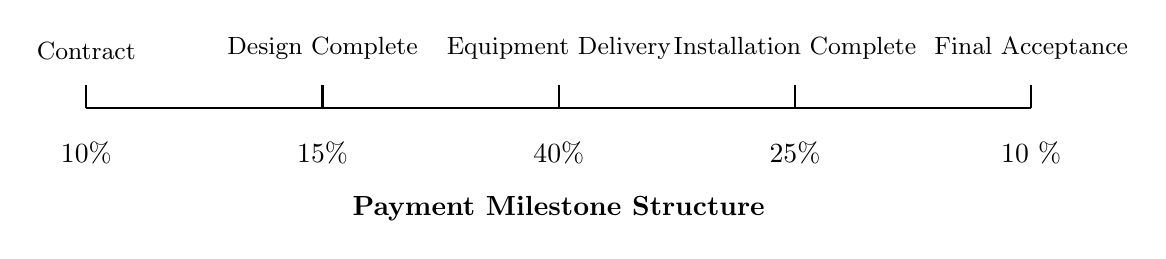
\begin{tikzpicture}
    % Payment milestones
    \draw[thick] (0,0) -- (12,0);

    \foreach \x/\milestone/\percent in {
        0/{Contract}/10,
        3/{Design Complete}/15,
        6/{Equipment Delivery}/40,
        9/{Installation Complete}/25,
        12/{Final Acceptance}/10
    } {
        \draw[thick] (\x,0) -- (\x,0.3);
        \node[above] at (\x,0.5) {\small\milestone};
        \node[below] at (\x,-0.3) {\percent\%};
    }

    \node[below] at (6,-1) {\textbf{Payment Milestone Structure}};
\end{tikzpicture}
\caption{Proposed payment schedule}
\end{figure}

\section{Proposal Evaluation Process}

\subsection{Stage 1: Compliance Review}

\begin{itemize}
    \item Verify all mandatory criteria met
    \item Check proposal completeness
    \item Confirm required documentation
    \item Initial risk assessment
\end{itemize}

\subsection{Stage 2: Technical Evaluation}

\begin{requirement}{TEND-005}{Technical evaluation by expert panel}

\begin{itemize}
    \item Detailed scoring against matrix
    \item Technical clarification meetings
    \item Reference site visits
    \item Proof of concept demonstrations
\end{itemize}

\subsection{Stage 3: Commercial Evaluation}

\begin{itemize}
    \item Total cost of ownership analysis
    \item Value for money assessment
    \item Payment term negotiations
    \item Contract term review
\end{itemize}

\subsection{Stage 4: Final Selection}

\begin{itemize}
    \item Shortlist presentations (3-4 bidders)
    \item Best and final offer process
    \item Executive approval
    \item Contract negotiations
\end{itemize}

\section{Contract Framework}

\subsection{Key Contract Terms}

\begin{table}[H]
\centering
\begin{tabularx}{\textwidth}{@{}lX@{}}
\toprule
\textbf{Term} & \textbf{Requirement} \\
\midrule
Performance Bond & 10\% of contract value \\
Liquidated Damages & £5,000 per week delay \\
Warranty Period & 24 months from acceptance \\
Defects Liability & 12 months from completion \\
Insurance & Professional indemnity £5M \\
IP Rights & Client ownership of custom work \\
\bottomrule
\end{tabularx}
\caption{Key commercial terms}
\end{table}

\subsection{Service Level Agreement}

Post-warranty support requirements:

\begin{itemize}
    \item \textbf{Response Times}:
        \begin{itemize}
            \item Critical: 4 hours
            \item Major: Next business day
            \item Minor: 5 business days
        \end{itemize}
    \item \textbf{Uptime Target}: 99.5\% availability
    \item \textbf{Maintenance}: Quarterly preventive visits
    \item \textbf{Remote Support}: 24/7 helpdesk
    \item \textbf{Spare Parts}: Guaranteed availability 7 years
\end{itemize}

\section{Risk Management}

\subsection{Procurement Risks}

\begin{table}[H]
\centering
\begin{tabularx}{\textwidth}{@{}lXl@{}}
\toprule
\textbf{Risk} & \textbf{Mitigation} & \textbf{Impact} \\
\midrule
Limited competition & Early market engagement & High \\
Technology obsolescence & Future-proof specifications & Medium \\
Integration complexity & Proven integrator selection & High \\
Budget overrun & Fixed price contract & Medium \\
Schedule delay & Liquidated damages & Medium \\
\bottomrule
\end{tabularx}
\caption{Key procurement risks and mitigations}
\end{table}

\subsection{Vendor Management}

\begin{itemize}
    \item Regular progress reviews
    \item Stage gate approvals
    \item Independent technical advisor
    \item Change control process
    \item Dispute resolution procedure
\end{itemize}

\begin{center}
\begin{tikzpicture}
\node[rectangle, draw=dreamlabPrimary, fill=dreamlabLight!20, text width=14cm, inner sep=15pt, rounded corners] {
\centering
\textbf{\large\color{dreamlabPrimary}Systems Integrator Tender Summary}\\[0.5cm]
Our comprehensive tender process ensures selection of a world-class systems integrator capable of delivering this ambitious project. Through rigorous evaluation criteria, clear specifications, and robust commercial terms, we will identify a partner who combines technical excellence with project delivery expertise to create one of the world's most advanced immersive research facilities.
};
\end{tikzpicture}
\end{center}